\section{Rsnap}
\graphicspath{{content/7-solution/3-rsnap/images/}}

\subsection{Interface}
présentation de l'interface :
\begin{itemize}
  \item design joli et adaptative
  \item student side
  \item prof side
  \item arrangement des missions + ouverture successive
  \item passage rsnap/snap
\end{itemize}

\subsection{Implémentation}
Comme expliqués en section \ref{rails}, Rails possède une architecture Model-Vue-Controleur (MVC). Cette section va présenter l'application en se basant sur ce modèle d'architecture. La première partie explique donc le modèle, ensuite les contrôleurs sont discutés. Enfin les vues sont présentées.

\subsubsection{Modèles}
Les différents concepts utiles pour développer l'application sont ceux représentés par les différents modèles. Ceux-ci sont présentés sur la figure \ref{fig:models}.

\begin{figure}
 \begin{center}
   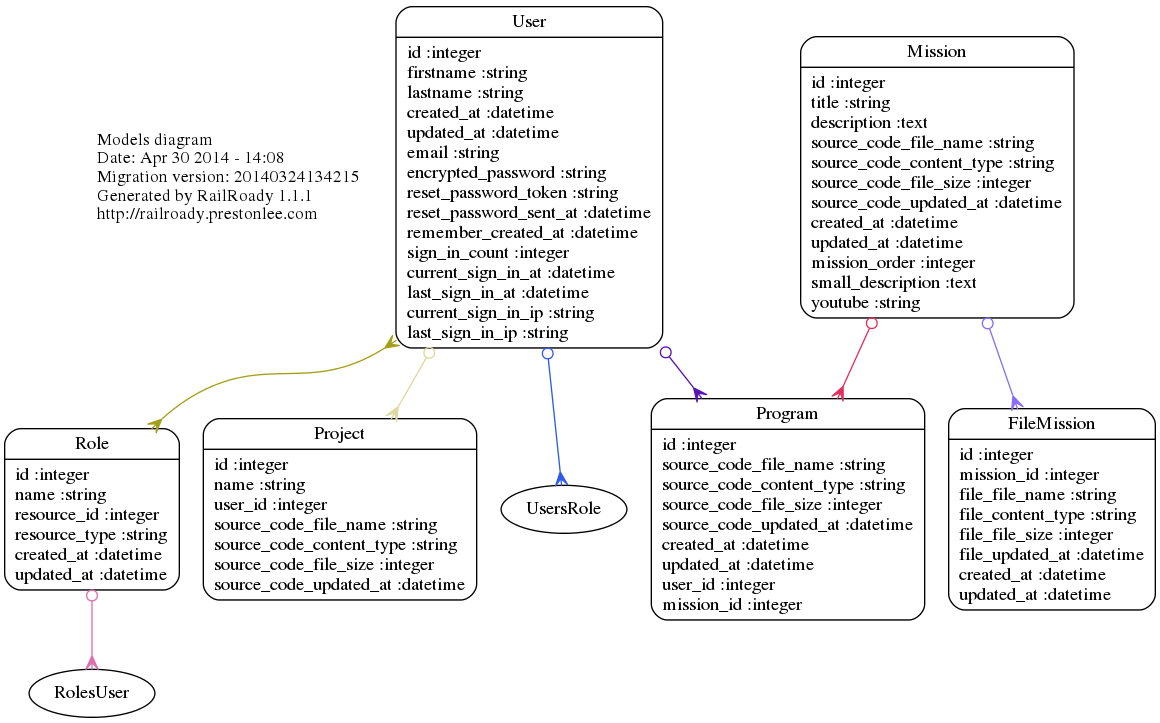
\includegraphics[width=\textwidth]{models_complete}
   \caption{Modèles de Rsnap}
   \label{fig:models}
 \end{center}
\end{figure}

\paragraph{\texttt{User}} L'utilisateur contient les informations nécessaires à l'identifier (\texttt{firstname}, \texttt{email} \ldots) et les informations pour s'authentifier (\texttt{encrypted\_password}, \texttt{current\_sign\_in\_ip}, \ldots). L'utilisateur peut posséder plusieurs rôles, programmes et projets.

\paragraph{\texttt{Rôle}} Les rôles permettent de donner des attributs à un utilisateur. Ce modèle a été généré automatiquement par Rolify \ref{rolify}. Dans le cas de Rsnap, deux types d'utilisateurs ont été créés : \texttt{admin} et \texttt{teacher}. Ces deux rôles sont globaux et donc ne sont pas rattachés à une ressource spécifique.%TODO dans futur Works: role teacher sur ressource students_group

Les rôles seront utiles en conjonction avec les autorités \ref{authority} pour donner des droits supplémentaires à ces types d'utilisateurs.

\paragraph{\texttt{Mission}} Les missions représentent tout ce qui est nécessaire pour avoir un exercice. Une mission comporte donc un titre, une description avec des images et une vidéo pour expliquer à l'étudiant ce qu'il devra faire. De plus elle comporte le code source initial de l'exercice. Généralement, celui-ci contient le squelette initial du programme pour l'étudiant et les tests pour vérifier le programme. 

\paragraph{\texttt{FileMission}} Les fichiers liés à une mission sont les différentes images qui compose la description. %TODO dans furture work : on peut imaginer rajouter la possibilité de mettre d'autre style de fichier dedans : ex. PDF, slide de cours...

\paragraph{\texttt{Program}} Un programme contient la solution d'un étudiant pour une mission. Ils comportent uniquement le code source de l'étudiant.

\paragraph{\texttt{Project}} Les projets sont identiques aux programmes mais ne sont pas liés à une mission. Ils comportent donc le nom du projet en plus du code source.

\paragraph{Exemple} \texttt{Program} est un bon exemple de modèle Rails (code source \ref{lst:model-program}). Seules les fonctionnalités qu’Active Record \ref{active-record} ne sait pas déduire de lui-même sont présentes. Le modèle contient donc uniquement :
\begin{itemize}
  \item le nom des modèles avec qui il est associé et la cardinalité de la relation (\lstinline[language=Rails]{belongs_to} ligne 5-6) ;
  \item la validation de certains attributs pour qu'ils respectent certaines contraintes (\lstinline[language=Rails]{validates} ligne 13-15) ;
  \item des méthodes de classes pour simplifier les requêtes au modèle (\lstinline[language=Rails]{scope},  \lstinline[language=Rails]{self.*} ligne 17-23).
\end{itemize}

Comme c'est visible pour les \lstinline[language=Rails]{scope} à la ligne 17-19, Active Record permet de faire des requêtes SQL directement en Ruby. 
\lstinputlisting[language=Rails, firstline=21, caption={Modèle \texttt{Program}}, label=lst:model-program]{content/7-solution/3-rsnap/listings/program.rb}

\subsubsection{Controlleurs}
Les contrôleurs donnent accès à différentes ressources. La figure \ref{fig:controllers} montre la liste des contrôleurs implémentés pour cette application. La majorité de ceux-ci se rapporte directement à un modèle spécifique. Il existe néanmoins certaines ressources différentes telles que : 
\begin{itemize}
  \item les pages statiques (\texttt{HomeController}) ;
  \item l'ordonnancement des missions (\texttt{SortMissionsController}) ; 
  \item la création d'un programme depuis une mission (\texttt{InitializationMissionController}) ;
  \item les ressources utiles à l'affichage de Snap! (\texttt{SnapAssetsController}).
\end{itemize}
\begin{figure}
 \begin{center}
   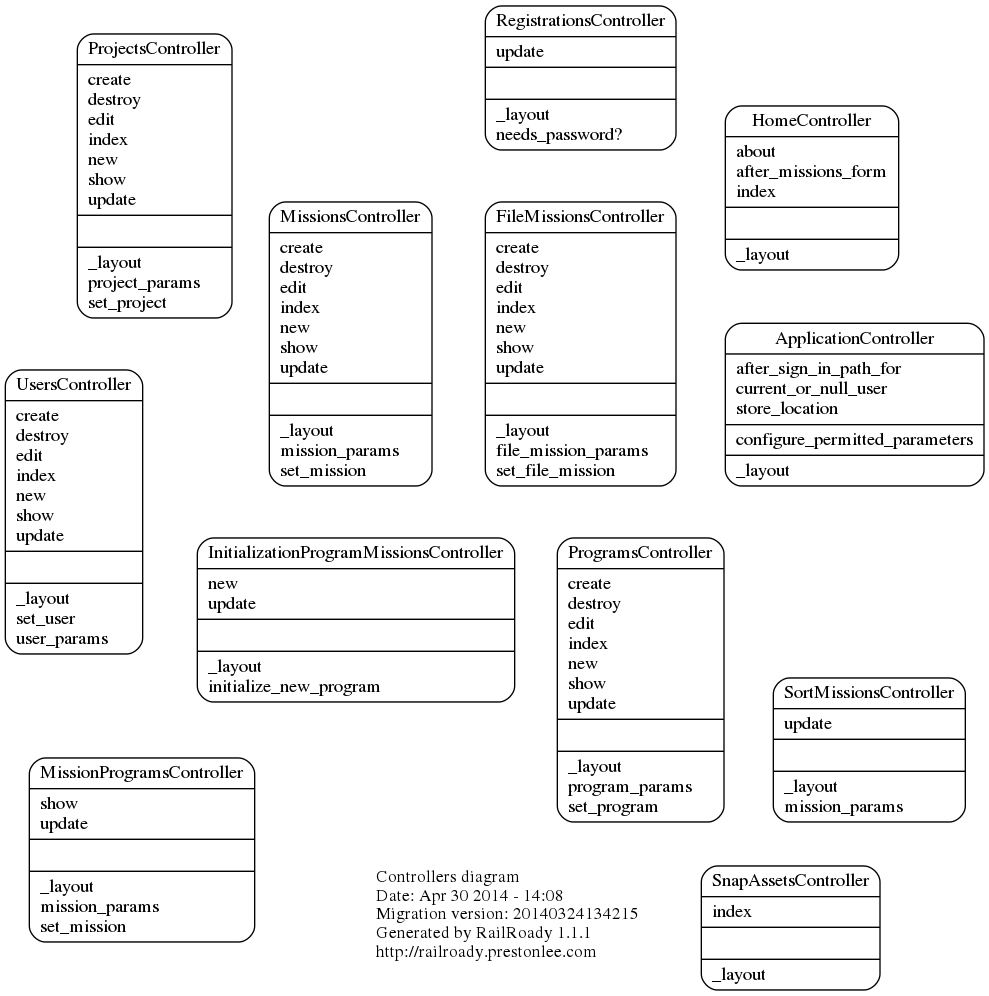
\includegraphics[width=\textwidth]{controllers_complete}
   \caption{Controlleurs de Rsnap}
   \label{fig:controllers}
 \end{center}
\end{figure}

Comme expliqué dans la section \ref{controleur}, les méthodes accessibles sont définies dans \texttt{routes.rb}. Les contrôleurs ont des tous des ressources RESTfull exceptées \texttt{HomeController}. Ceci est visible dans \texttt{routes.rb} ou en regardant les fonctions publiques disponibles dans les contrôleurs sur la figure \ref{fig:controllers}.

\paragraph{Exemple}
L'extrait du contrôleur \texttt{MissionsController} \ref{lst:controller-mission} montre l'usage classique d'un contrôleur. 

\lstinputlisting[language=Rails, linerange={1-5,10-34,52-62}, caption={Extrait du controlleur \texttt{MissionsController}}, label=lst:controller-mission]{content/7-solution/3-rsnap/listings/missions_controller.rb} %TODO verifier les ranges des lignes

Grâce au méta-programmation, \lstinline[language=Rails]{authorize_actions_for Mission} permet de rajouter, sur toutes les méthodes RESTfull, une vérification de ce que peut réaliser ou pas l'utilisateur courant. Ces vérifications sont injectées dans les autorités \ref{autority}. De plus, la méthode \lstinline[language=Rails]{before_filter} permet de réaliser une action supplémentaire avant chaque appel de fonction. Ici, excepté pour l'action \texttt{show} et \texttt{index} qui peuvent être publique, il faut que l'utilisateur soit authentifié pour que l'application puisse par après vérifier ses droits. %TODO pas claire sur la fin tu commences par les exceptions

Dans une méthode du contrôleur accessible via les routes, plusieurs actions sont à implémenter :
\begin{enumerate}
  \item traiter, si nécessaire, les paramètres fournis. Ceux-ci se trouvent dans \lstinline[language=Rails]{param} ;
  \item Assigner les variables d'instance que nécessitera la vue pour s'afficher correctement ;
  \item Exécuter le rendu de la page. Si la vue a le même nom que la méthode, cette étape est facultative.
\end{enumerate}

\subsubsection{Vue}
\label{vues}
Les vues sont écrites en haml \ref{haml}. L'exemple de code \ref{lst:vue-user-index} avec \ref{lst:vue-user-partial} montre comment est représenté la vue servant à lister tout les utilisateurs \ref{fig:vue-users}.

\lstinputlisting[language=haml, caption={Vue \texttt{index} des utilisateurs}, label=lst:vue-user-index]{content/7-solution/3-rsnap/listings/index.html.haml}
Le code source \ref{lst:vue-user-index} présente comment sont utilisé les variables d'instance créées par le contrôleur. Par exemple, la variable \texttt{@title} sert de titre 1.

\lstinputlisting[language=haml, caption={Vue d'une ligne \texttt{\_user} représentant un utilisateur}, label=lst:vue-user-partial]{content/7-solution/3-rsnap/listings/_user.html.haml}
De plus, Rails permet de faire le rendu d'un autre fichier de manière élégante. La ligne 14 du code source \ref{lst:vue-user-index} permet d'exécuter le rendu sur tous les éléments de la collection \texttt{users} grâce au fichier \ref{lst:vue-user-partial}

Les connaisseurs de Bootstrap \ref{bootstrap} auront reconnu l'usage intensif des classes de style qu'il propose. L'adaptativité de cet outil est visible sur la capture d'écran \ref{fig:vue-users}. En effet, le menu supérieur a été réduit, car la taille de l'écran était trop petite pour accueillir le menu en entier.

\begin{figure}
  \begin{center}
    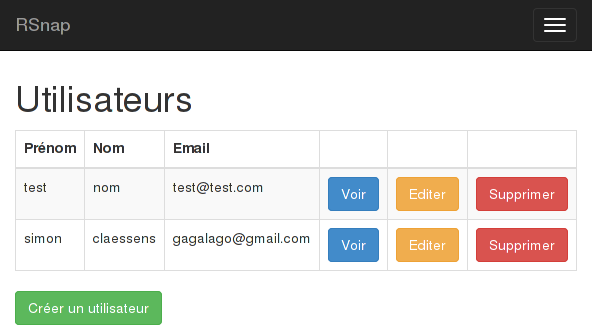
\includegraphics[width=.8\textwidth]{users}
    \caption{Affichage de la vue présentée par le code source \ref{lst:vue-user-index} et \ref{lst:vue-user-partial}}
    \label{fig:vue-users}
  \end{center}
\end{figure}

\subsection{Choix techniques}
expliquer les différentes possibilités de stockage (fichier et site) prix, fonctionnalité...

\subsection{Utilisation}
Pour utiliser la plateforme, il faut tout d'abord s'enregistrer dessus. Ensuite, suivant le profil, différentes actions sont possibles. L'utilisateur normal peut uniquement résoudre les missions dans l'ordre proposé par les professeurs. Les professeurs peuvent aussi créer des missions. Cette section présente l'utilisation de la plateforme.
%TODO faire des schémas/scénario avec les screenshot + tous les screenshot en annexe

\paragraph{Professeur}
Un professeur pour réaliser un cours de programmation doit pouvoir faire les choses suivante:
\subparagraph{Créer des missions} Pour créer une nouvelle mission (figure \ref{fig:mission-create}), le professeur doit se rendre sur la page qui liste toutes les missions, ensuite il peut cliquer sur le bouton en bas de page "Nouvelle mission". La page suivante permet de renseigner les informations sur la mission : titre, description et explication de la mission, vidéo d'explication \ldots Il reste enfin à créer la mission proprement dite. Pour cela, lorsque le professeur clique sur le bouton "Créer une mission", il est redirigé vers l'interface de Snap!. Il peut alors créer tout ce qui est nécessaire à la réalisation et au test de la mission. Avant de sauver, il ne doit pas oublier de cacher les blocs et les scriptes qui ne doivent pas être visibles des étudiants.
\begin{figure}
  \begin{center}
    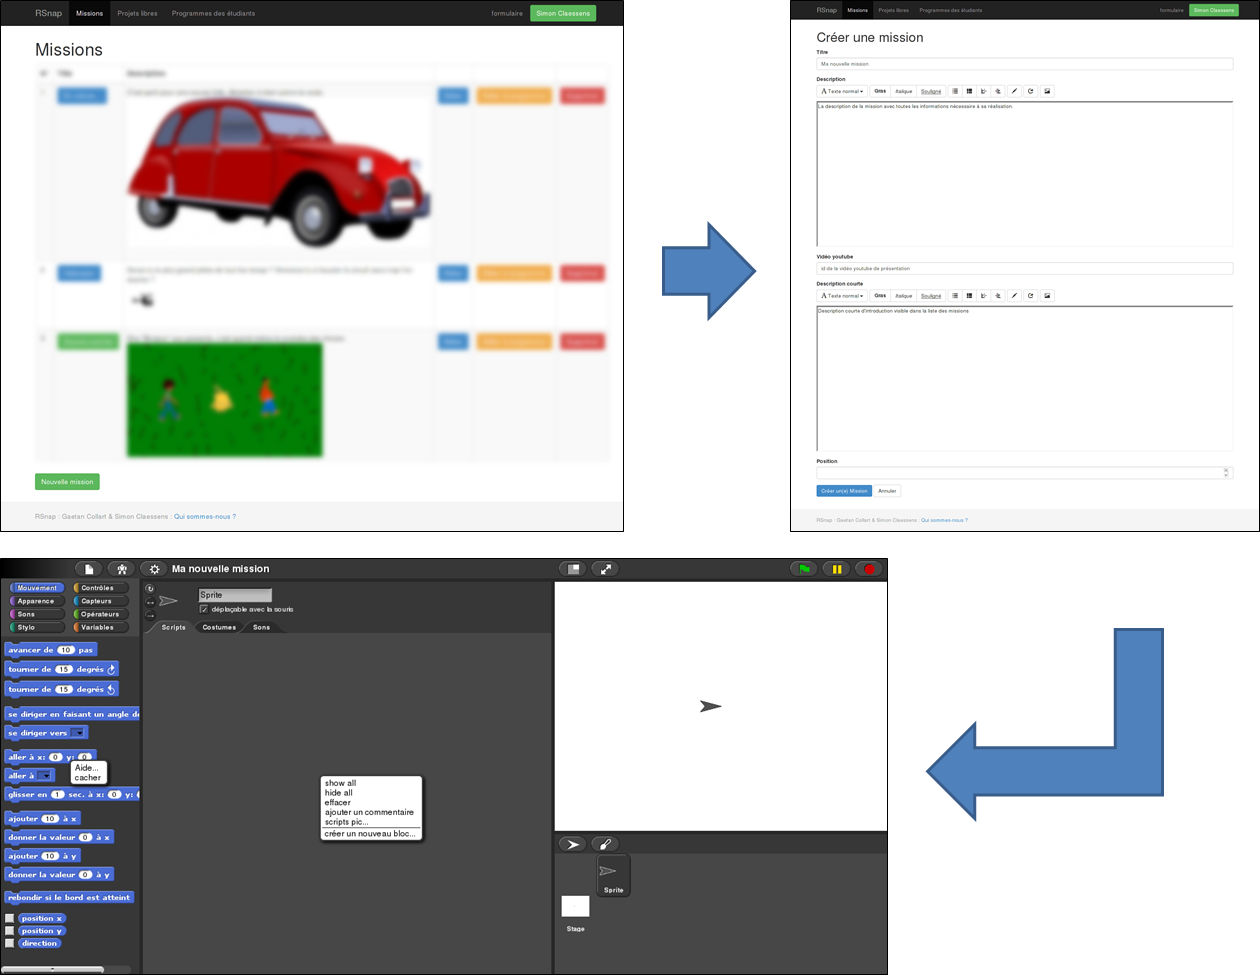
\includegraphics[width=.9\textwidth]{mission-create}
    \caption{Création d'une mission}
    \label{fig:mission-create}
  \end{center}
\end{figure}

\subparagraph{Ordonner les missions} Pour ordonner les missions (figure \ref{fig:mission-order}) dans un ordre pédagogique, il suffit de glisser les missions dans la liste.
\begin{figure}
  \begin{center}
    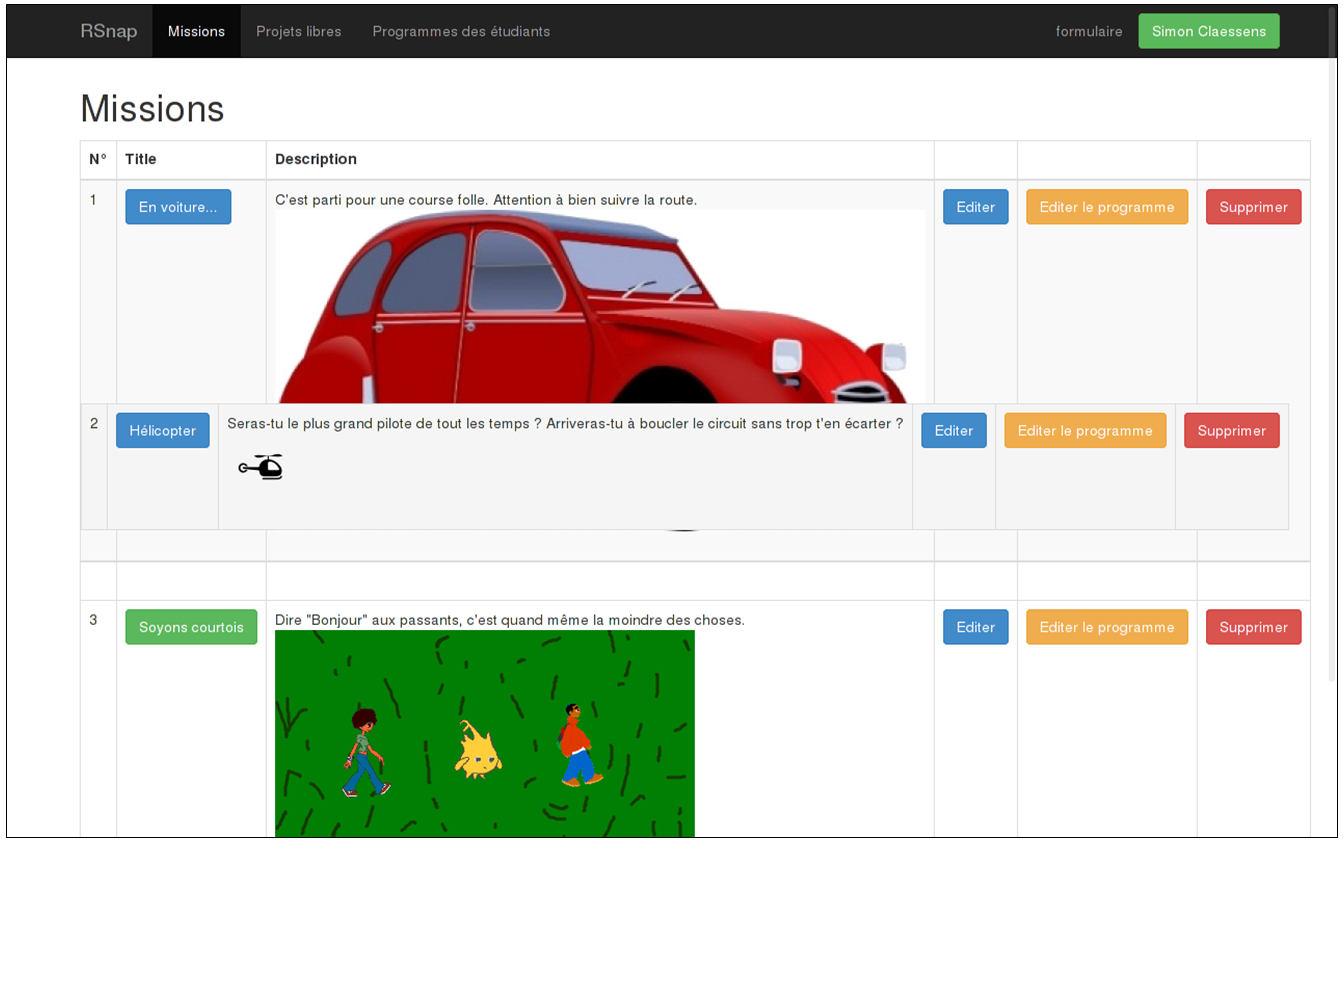
\includegraphics[width=.9\textwidth]{mission-order}
    \caption{Ordonner les missions}
    \label{fig:mission-order}
  \end{center}
\end{figure}

\subparagraph{Corriger les soumissions de ses étudiants} Pour corriger les soumissions de ses étudiants (figure \ref{fig:program-correction}), le professeur se rend sur la page des programmes. À ce moment, il voit le programme qu'il désire corriger. Le programme de l'étudiant s'ouvrira dans l'interface Snap! Il pourra alors rajouter des commentaires.
\begin{figure}
  \begin{center}
    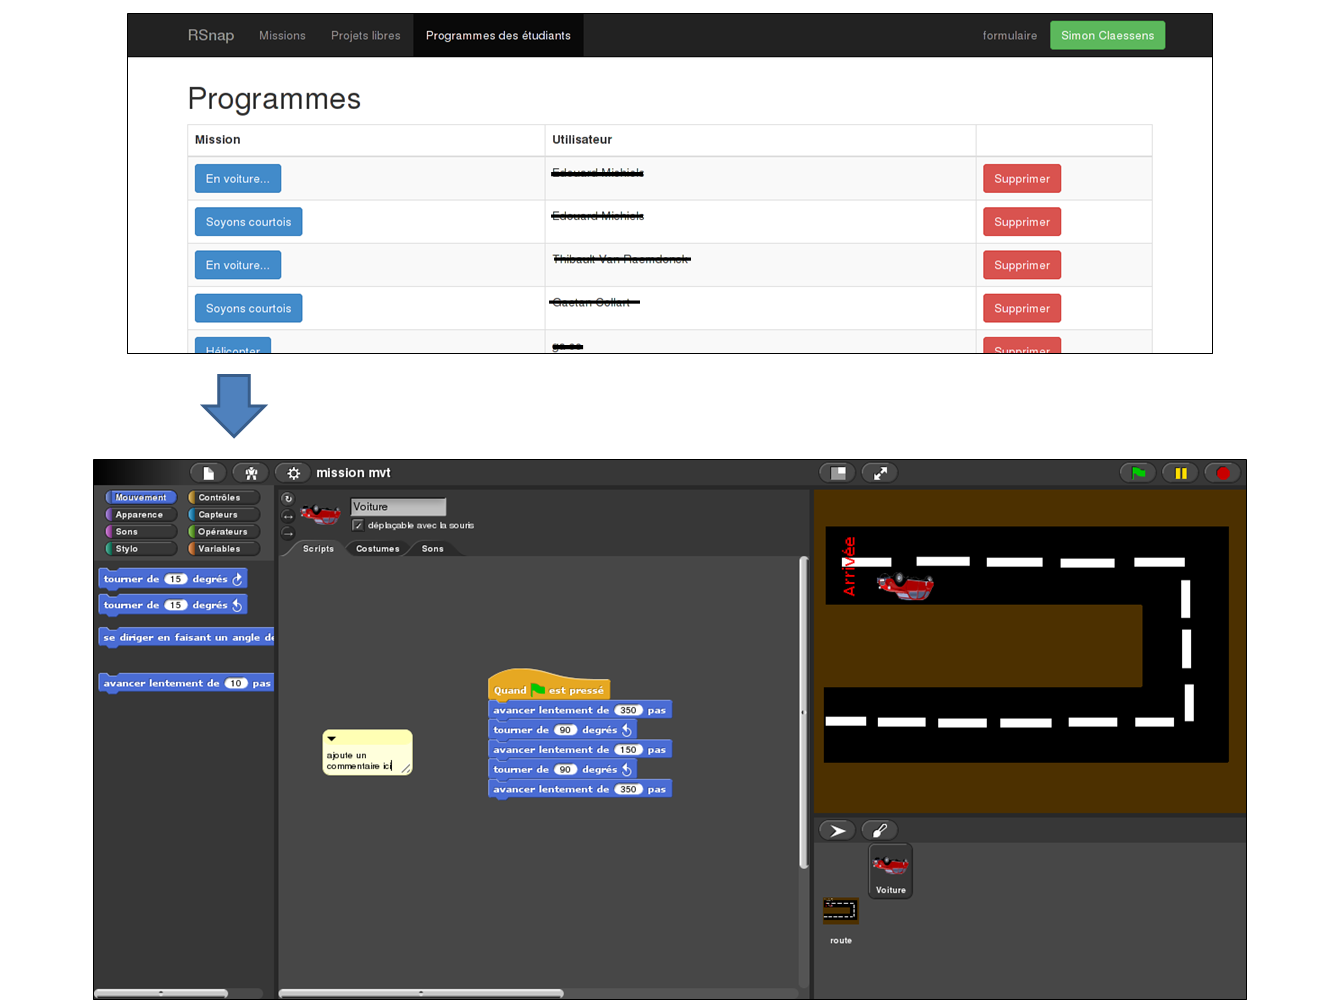
\includegraphics[width=.9\textwidth]{program-correction}
    \caption{Correction d'un programme}
    \label{fig:program-correction}
  \end{center}
\end{figure}

\paragraph{Étudiant}
Un étudiant veux pouvoir réaliser les opérations suivantes :
\subparagraph{Réaliser une mission} L'étudiant peut réaliser une mission (figure \ref{fig:program-creation}) en cliquant sur le nom de la mission. 

Deux possibilité s'offre a lui. Soit le bouton est bleu, ce qui signifie que l'étudiant a déjà commencé la mission, il la va donc la continuer là où il s'était arrêter. Soit le bouton est vert et dans ce cas l'étudiant commence la mission depuis le départ.

Dans les deux cas, il se retrouve sur l'interface de Snap! où il résout la mission.
\begin{figure}
  \begin{center}
    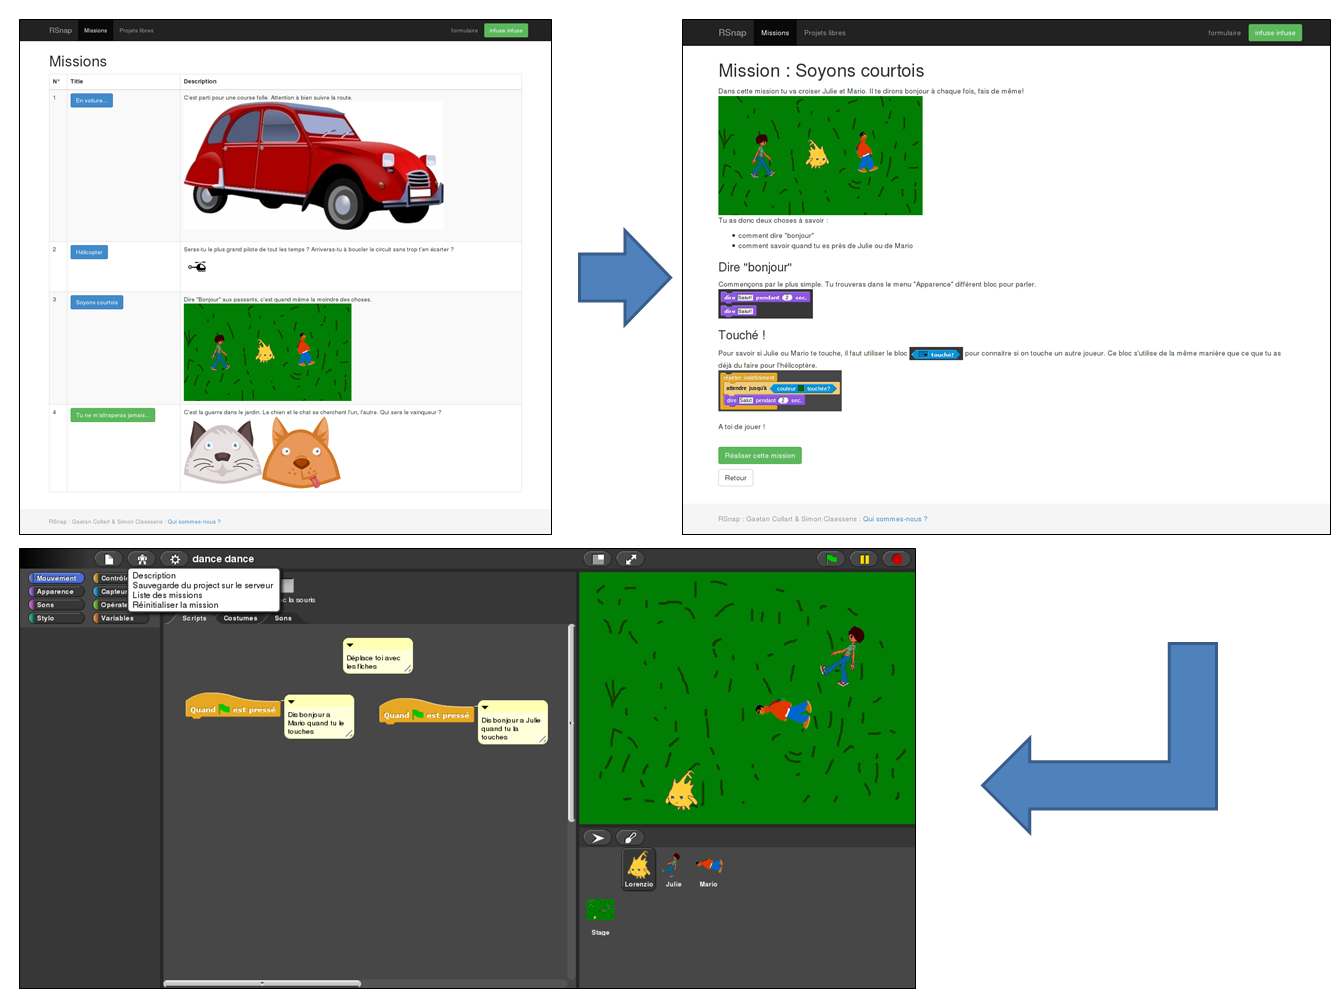
\includegraphics[width=.9\textwidth]{program-creation}
    \caption{Réalisation d'une mission}
    \label{fig:program-creation}
  \end{center}
\end{figure}

\subparagraph{Réaliser un projet libre} Si l'étudiant a envie de créer quelque chose, il peut aller dans projet libre. Il pourra alors utiliser Snap! à son plein potentiel et pourra laisser libre court à son imagination pour créer le programme de ses rêves.
